
\section{Resultados}

\subsection{Visión General}

Hemos investigado el uso de la biología de sistemas para entender mejor el fenotipo diabetes materna. En esta sección presentaremos los resultados del análisis de la red de genes relacionados con el fenotipo a partir de datos de interacción proteína-proteína descargados de STRINGdb con el propósito de estudiar la relación entre la diabetes materna y el gen GNB3.

A continuación procederemos a detallar los resultados obtenidos al ejecutar nuestro flujo de trabajo.

\subsection{Red de interacción}

Al descargar la lista de genes implicados en el fenotipo de estudio, observamos que la cantidad de enfermedades asociadas son 31 y los genes son 43. Hemos generado la red de interacción entre estos genes para obtener la cantidad de nodos e interacciones entre ellos. En la Tabla~\ref{table:nodes_edges_count} se puede observar la cantidad de nodos (genes) y edges (interacciones) de la red sin incluir el gen GNB3 e incluyendo al gen para hacer la red.


\begin{table}[h]
	\centering
	\caption{Cantidad de nodos e interacciones: Se ha creado la red de interacciones de los genes relacionados con el fenotipo y otra red añadiendo al gen de estudio. Finalmente, se ha obtenido la cantidad de nodos y edges de cada red.}
	\label{table:nodes_edges_count}
	\begin{tabular}{|c|c|c|}
		\hline
		\textbf{Red} & \textbf{Nodos} & \textbf{Edges} \\ \hline
		Sin GNB3 & 43    & 272   \\ \hline
		Con GNB3 & 44    & 276  \\ \hline
	\end{tabular}

\end{table}

La red generada por stringdb usando los genes asociados a la diabetes materna y el GNB3 se pude observar en la Figura~\ref{fig:network}.

\begin{figure}[h!]
	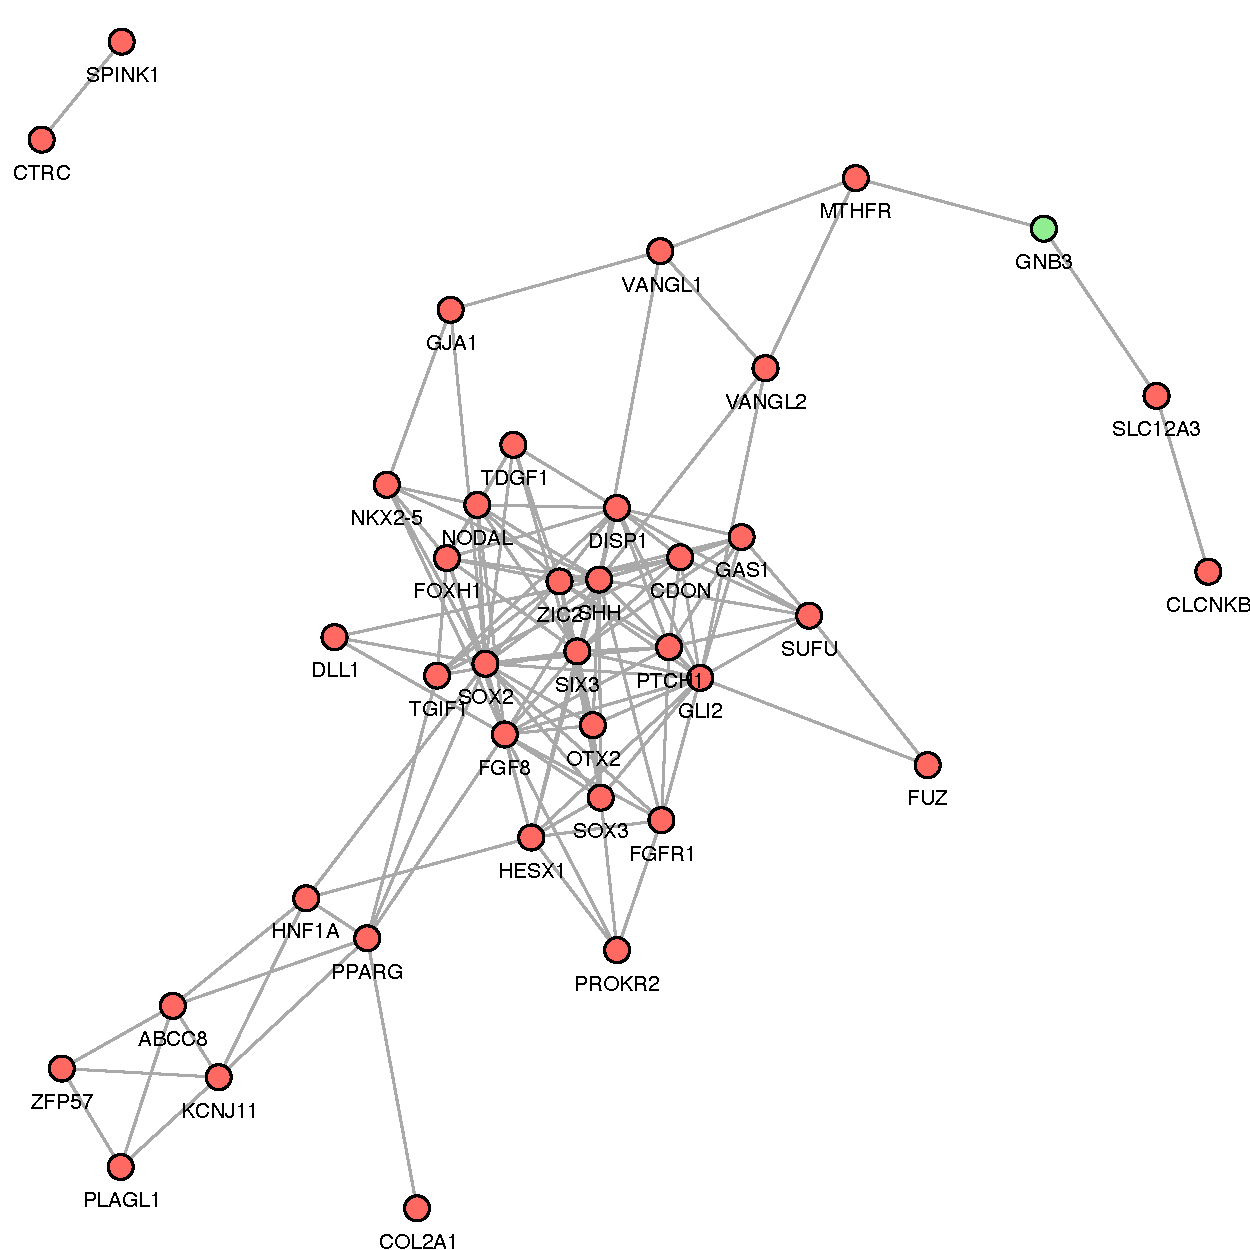
\includegraphics[width=0.9\textwidth]{figures/network.pdf}
	\caption{Red de Interacción: Se observan las interacciones entre los genes asociados al fenotipo de estudio y el gen GNB3. Los nodos en rojo representan los genes asociados al fenotipo, mientras que el nodo verde representa al GNB3.}
	\label{fig:network}
\end{figure}

\subsection{Detección de comunidades}

Hemos detectado las comunidades de la red obtenida en el paso anterior, usando el método ``edge betweenness'' descrito en la sección de métodos. Obtuvimos cinco comunidades a partir de la red de interacciones. El GNB3 se encuentra presente en una comunidad con otros dos nodos, los genes SLC12A3 y el CLCNKB, como puede observarse en la Figura~\ref{fig:comunidad}.

\begin{figure}[h!]
	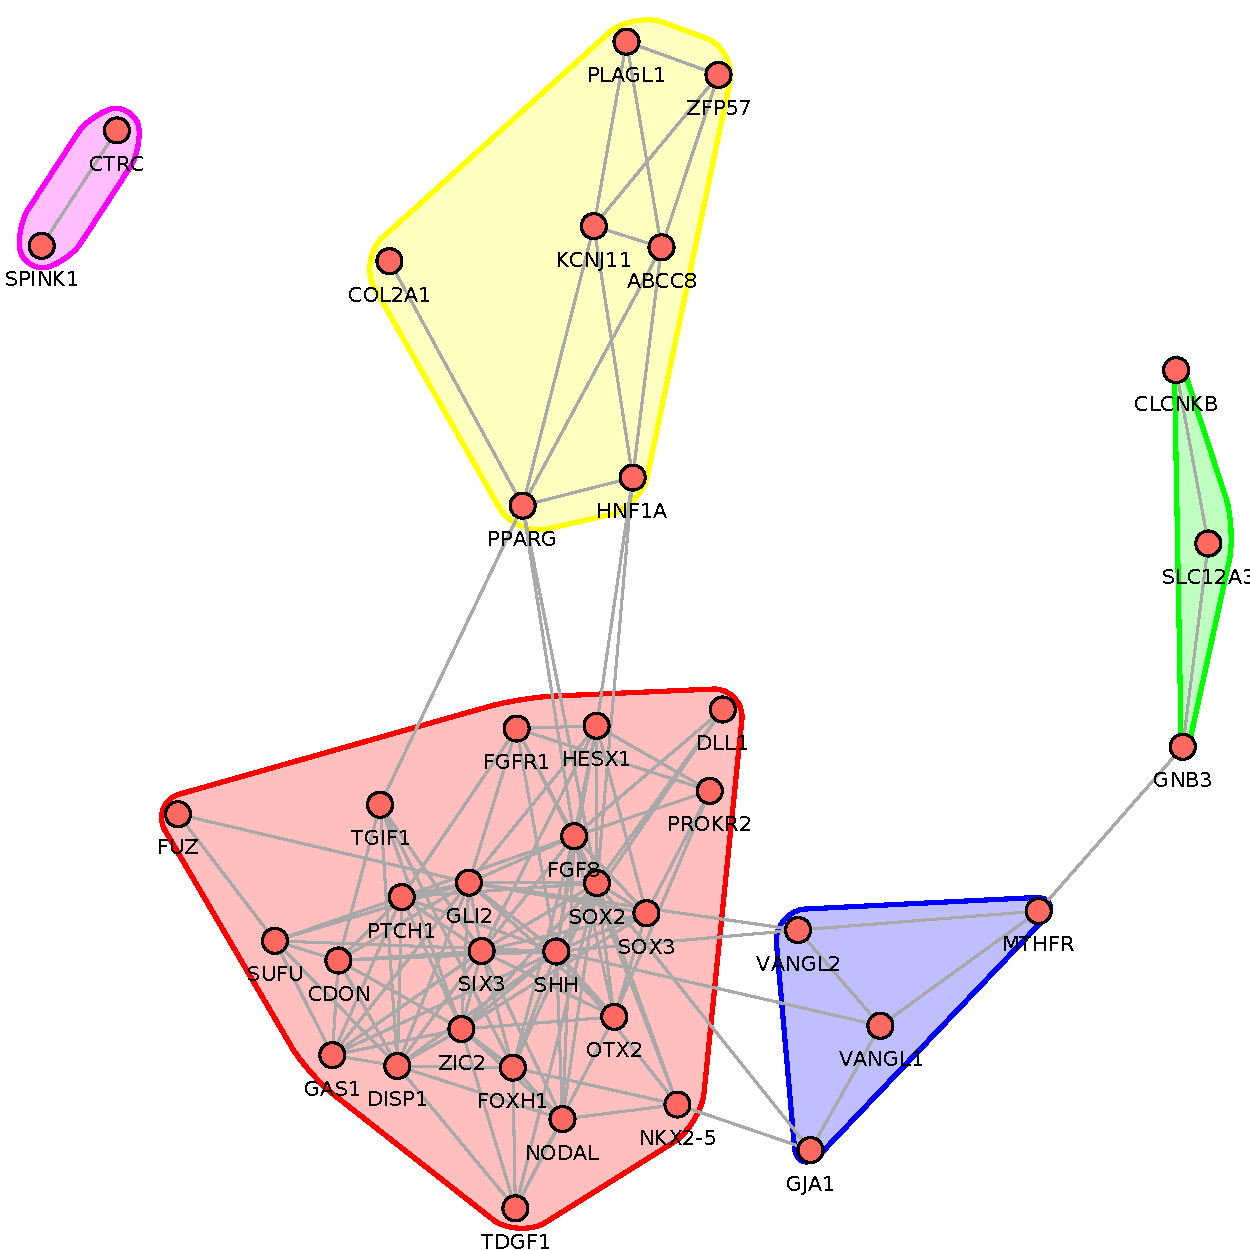
\includegraphics[width=0.9\textwidth]{figures/comunidades.pdf}
	\caption{Detección de comunidades: Se representa la clusterización de los nodos en cinco comunidades.}
	\label{fig:comunidad}
\end{figure}

\subsection{Enriquecimiento funcional}

Una vez detectada la comunidad a la que pertenece el GNB3 en la red de estudio, hemos obtenido el enriquecimiento funcional para los tres genes pertenecientes a la comunidad.  Filtrando aquellos resultados en los que aparece el gen GNB3, el análisis demostró un enriquecimiento para el fenotipo HPO de anormalidad de la visión, con un p-valor de 0.00021, como se puede observar en la Tabla~\ref{table:enriquecimiento1}

\begin{table}[h]
	\centering
	\caption{Enriquecimiento funcional de la comunidad del gen GB3: Se observa el único resultado para el gen de interés.}
	\label{table:enriquecimiento1}
	\begin{tabular}{|c|c|c|c|c|c|}
		\hline
		\textbf{Preferred Names} & \textbf{Description} & \textbf{P-value} & \textbf{fdr} & \textbf{Category} & \textbf{Term} \\ \hline
		GNB3, CLCNKB, SLC12A3 & Abnormality of vision    & 0.00021 & 0.0197&  HPO & HP:0000504 \\ \hline

	\end{tabular}

\end{table}

\subsection{Propagación de la red}

Hemos realizado la propagación de la red añadiendo 16 nodos más, que interaccionan con los tres genes pertenecientes a la comunidad del gen GNB3. A continuación, hemos procedido a realizar el enriquecimiento funcional incluyendo los nuevos genes. En este caso, el gen de interés apareció implicado en 96 procesos, de los cuales se muestran aquellos relacionados con la regulación de insulina y glucagón en la Tabla~\ref{table:enriquecimiento2}. Se puede observar que, en todos los casos representados, hay un enriquecimiento significativo en términos relacionados con RCTM, que ha sido introducido en la sección de métodos.


\begin{table}[h]
	\centering
	\caption{Enriquecimiento funcional de la comunidad del gen GB3 expandida: Se observan los resultados que incluyen al gen GNB3 y que incluyen mecanismos relacionados con la insulina o el glucagón. Todos los resultados son de la categoría RCTM.}
	\label{table:enriquecimiento2}
	\begin{tabular}{|c|c|c|c|}
		\hline
		 \textbf{Description} & \textbf{P-value} &\textbf{ fdr }&  \textbf{Term} \\ \hline
		 Regulation of insulin secretion   & 9.38e-30 & 1.05e-27 &   HSA-422356 \\ \hline
		 Glucagon-like Peptide-1 (GLP1) regulates insulin secretion  & 3.57e-30 & 5.44e-28  & HSA-381676 \\ \hline
		 Adrenaline,noradrenaline inhibits insulin secretion & 3.88e-29 & 3.28e-27  & HSA-400042 \\ \hline
		 Glucagon-type ligand receptors & 2.51e-31 & 5.73e-29  & HSA-420092 \\ \hline
		 Glucagon-like Peptide-1 (GLP1) regulates insulin secretion & 3.57e-30 & 5.44e-28  & HSA-381676 \\ \hline
		 Glucagon signaling in metabolic regulation & 1.31e-25 & 6.95e-24  & HSA-163359 \\ \hline
		 Synthesis, secretion, and inactivation of Glucagon-like Peptide-1 (GLP-1) & 1.33e-06 & 4.39e-05  & HSA-381771 \\ \hline
	\end{tabular}

\end{table}

Después de haber presentado los resultados, la discusión de los mismos seguirá en la próxima sección.
